%%%%%%%%%%%%%%%%%%%%%%%%%%%%%%%%%%%%%%%%%%%%%%%%%%%%%%%%%%%%%%%%%%%%%
%
%  This is a sample LaTeX input file for your contribution to 
%  the MC2013 conference. Modified by R.C. Martineau at INL from A. 
%  Sood at LANL, from J. Wagner ORNL who obtained the original class 
%  file by Jim Warsa, LANL, 16 July 2002}
%
%  Please use it as a template for your full paper 
%    Accompanying/related file(s) include: 
%       1. Document class/format file: mc2013.cls
%       2. Sample Postscript Figure:   figure.eps
%       3. A PDF file showing the desired appearance: template.pdf 
%    Direct questions about these files to: richard.martinea@inl.gov
%
%    Notes: 
%      (1) You can use the "dvips" utility to convert .dvi 
%          files to PostScript.  Then, use either Acrobat 
%          Distiller or "ps2pdf" to convert to PDF format. 
%      (2) Different versions of LaTeX have been observed to 
%          shift the page down, causing improper margins.
%          If this occurs, adjust the "topmargin" value in the
%          mc2013.cls file to achieve the proper margins. 
%
%%%%%%%%%%%%%%%%%%%%%%%%%%%%%%%%%%%%%%%%%%%%%%%%%%%%%%%%%%%%%%%%%%%%%


%%%%%%%%%%%%%%%%%%%%%%%%%%%%%%%%%%%%%%%%%%%%%%%%%%%%%%%%%%%%%%%%%%%%%
\documentclass{mc2013}
%
%  various packages that you may wish to activate for usage 
\usepackage{graphicx}
\usepackage{tabls}
\usepackage{afterpage}
\usepackage{cites}
\usepackage{amssymb}
\usepackage{amsfonts}
\usepackage{amsmath}
\usepackage{amsthm}
\usepackage[mathcal]{euscript}

%\usepackage{epsf}
%
%
% Insert authors' names and short version of title in lines below
%
\newcommand{\authorHead}      % Author's names here
   {Slattery, Wilson, and Pawlowski}  
\newcommand{\shortTitle}      % Short title here
   {Data Transfer Kit}  
%%%%%%%%%%%%%%%%%%%%%%%%%%%%%%%%%%%%%%%%%%%%%%%%%%%%%%%%%%%%%%%%%%%%%
%
%   BEGIN DOCUMENT
%
%%%%%%%%%%%%%%%%%%%%%%%%%%%%%%%%%%%%%%%%%%%%%%%%%%%%%%%%%%%%%%%%%%%%%
\begin{document}

%
%      Headers and Footers
\afterpage{%
\fancyhf{}%
\fancyhead[CE]{              
{\scriptsize \authorHead}}                                                
\fancyhead[CO]{               
{\scriptsize \shortTitle}}                  
%\lfoot{\scriptsize{
%International Conference on Mathematics and Computational Methods
%Applied to Nuclear Science \& Engineering (M\&C 2013), 
%\\ Sun Valley, Idaho, USA, May 5-9, 2013.}}%
\rfoot{\thepage/\totalpages{}}%

\pagestyle{fancy}
%\setlength{\topmargin}{-20pt}
}
 
\normalsize

\setlength{\baselineskip}{16.8pt}
\vspace{-3pt}

% 
% TITLE
%

\begin{center}
\textbf{\large \\%
THE DATA TRANSFER KIT: A GEOMETRIC RENDEZVOUS-BASED TOOL FOR
MULTIPHYSICS DATA TRANSFER
}
% 
% FIRST AUTHORS 
%
\\
\setlength{\baselineskip}{14pt}
\textbf{S.R. Slattery and P.P.H. Wilson} \\
Department of Engineering Physics \\
University of Wisconsin - Madison \\
1500 Engineering Dr., Madison, WI 53706 \\
sslattery@wisc.edu; wilsonp@engr.wisc.edu \\

% 
% SECOND AUTHORS (if not needed delete from here) 
%
\vspace{12pt} \textbf{R.P. Pawlowski} \\ Sandia National
Laboratories\footnote{Sandia National Laboratories is a multi-program
  laboratory managed and operated by Sandia Corporation, a wholly
  owned subsidiary of Lockheed Martin Corporation, for the
  U.S. Department of Energy\'s National Nuclear Security
  Administration under contract DE-AC04-94AL85000.} \\ P.O. Box 5800,
Albuquerque, NM 87185 \\ rppawlo@sandia.gov \\
%
% SECOND AUTHORS (to here)
%

\end{center}

%
% SET RAGGED RIGHT MARGIN
%
\raggedright


%%---------------------------------------------------------------------------%%
\section*{ABSTRACT} 
\begin{quote}
\begin{small}
The Data Transfer Kit (DTK) is a software component designed to
provide parallel data transfer services for arbitrary physics
components based on the concept of geometric rendezvous. The
rendezvous algorithm provides a means to geometrically correlate two
geometric domains that may be arbitrarily decomposed in a parallel
simulation. By repartitioning both domains such that they have the
same geometric domain on each parallel process, efficient and load
balanced search operations and data transfer can be performed at a
desirable algorithmic time complexity with low communication overhead
relative to other types of mapping algorithms. With the increased
development efforts in multiphysics simulation and other multiple mesh
and geometry problems, generating parallel topology maps for
transferring fields and other data between geometric domains is a
common operation. The algorithms used to generate parallel topology
maps based on the concept of geometric rendezvous as implemented in
DTK are described with examples using a conjugate heat transfer
calculation and thermal coupling with a neutronics code. In addition,
we provide the results of initial scaling studies performed on the
Jaguar Cray XK6 system at Oak Ridge National Laboratory for a
worse-case-scenario problem in terms of algorithmic complexity that
shows good scaling on $O(1 \times 10^4)$ cores for topology map
generation and excellent scaling on $O(1 \times 10^5)$ cores for the
data transfer operation with meshes of $O(1 \times 10^9)$ elements.


\emph{Key Words}: data transfer, multiphysics, rendezvous algorithm,
parallel computing
\end{small} 
\end{quote}

\setlength{\baselineskip}{14pt}
\normalsize

%%---------------------------------------------------------------------------%%
\Section{INTRODUCTION} 
\label{sec:intro}

In many physics applications, it is often desired to transfer fields
(i.e. degrees of freedom or other data) between geometric domains that
may or may not conform in physical space. In addition, for massively
parallel simulations, it is typical that geometric domains not only do
not conform spatially, but also that their parallel decompositions do
not correlate and are independent of one another due to physics-based
partitioning and discretization requirements. As an example, this
situation can occur in multiphysics simulations where physics fields
provide feedback between solution iterations \cite{Tautges_2009_2} or
parallel adaptive mesh simulations where fields must be moved between
meshes after refining and coarsening \cite{Edwards_2006}. It is
therefore desirable to have a set of tools to relate two geometric
domains of arbitrary parallel decomposition such that fields and other
data can be transferred between them.

The Data Transfer Kit (DTK) is a software component developed as part
of the Consortium for Advanced Simulation of LWR's (CASL)
\cite{u.s._department_of_energy_casl_2011} designed to provide
parallel services for mesh and geometry searching and data
transfer. The algorithms implemented in DTK are based on the concept
of geometric rendezvous as developed by Plimpton, Hendrickson, and
Stewart \cite{Plimpton_2004} originally implemented as part of the
SIERRA framework \cite{Stewart_2004}. Their work has been extended to
move towards a component design for use with arbitrary physics codes
such that varying representations of mesh, geometry, and fields are
able to access these services \cite{Chand_2008}. In addition, the
original mesh-based rendezvous algorithms have been expanded
to be used with both mesh and geometry representations of the
geometric domain. This document will briefly outline the rendezvous
algorithms as implemented in DTK. Examples of data transfer using a
conjugate heat transfer calculation and a thermal-neutronics type
coupling are provided. Parallel scaling results are also presented for
the mesh-based mapping algorithm for a worse-case-scenario problem
where communication costs are at a maximum.


%%---------------------------------------------------------------------------%%
\Section{GEOMETRIC RENDEZVOUS} 
\label{sec:geometric_rendezvous}

Relating two non-conformal meshes will ultimately require some type of
data evaluation algorithm to apply the data from one geometry to
another. To drive these evaluation algorithms, the target objects to
which this data will be applied must be located within the the source
geometry. In a serial formulation, efficient search structures that
offer logarithmic asymptotic time complexity are available to perform
this operation. However, in a parallel formulation, if these two
geometries are arbitrarily decomposed, geometric alignment is not
likely and a certain degree of communication will be required. A
geometric rendezvous manipulates the source and target geometries such
that all geometric operations have a local formulation.

A geometry that is providing data through function evaluations will be
referred to as the source geometry while the geometry that will be
receiving the data will be referred to as the target
geometry. Although explicitly formulated with a source mesh and target
vertices below, these concepts can be applied to geometric structures
beyond mesh and vertices.

\Subsection{Rendezvous Decomposition}
\label{subsec:rendezvous_algorithm}

The geometric rendezvous concept uses a global formulation for the
data transfer while maintaining a local formulation for the geometric
search operations by generating a secondary decomposition of the
geometric structures in the problem. This secondary decomposition is
generated by a geometry-based repartitioning for more load-balanced
searching algorithms. This repartitioning is shown in the example
presented in Figure~\ref{fig:rendezvous_example} where two meshes, one
of triangles and one of quadrilaterals, are decomposed into four
partitions that are not correlated to one another. To transfer data
between these meshes, each partition in both meshes will need to
communicate data to each partition in the other mesh due to their
geometric overlap. The rendezvous decomposition, shown on the right,
is a repartitioning of the source mesh in the transfer problem with
the partitioning information shared amongst both meshes. The
components of both meshes that are required for data transfer will be
gathered into this new partition.
\begin{figure}[htpb!]
  \centering 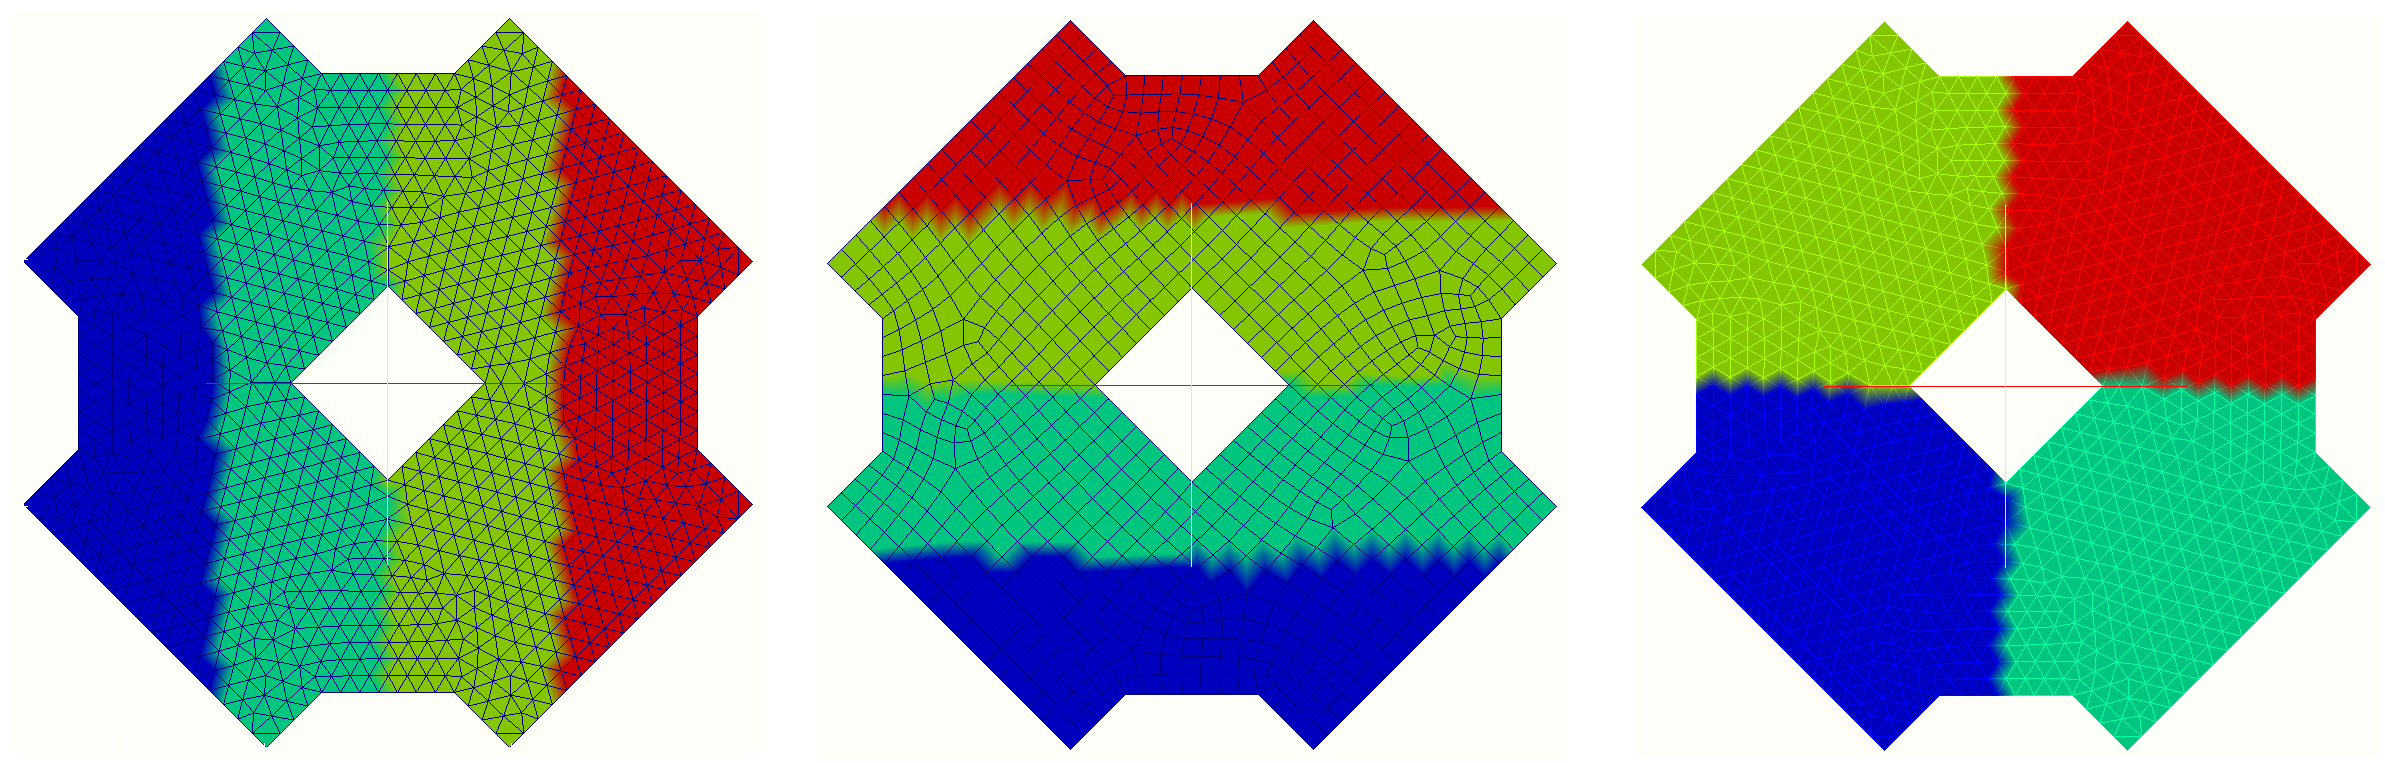
\includegraphics[width=6in]{rendezvous_example.png}
  \caption{Rendezvous decomposition example. A triangle mesh (left)
    and a quadrilateral mesh (center) are partitioned into 4 parallel
    domains as indicated by color. The rendezvous decomposition
    (right) is generated as a geometric-based repartitioning of the
    source mesh that permits load balanced geometric operations.}
  \label{fig:rendezvous_example}
\end{figure}

In DTK, the rendezvous algorithm developed by Plimpton
et. al. \cite{Plimpton_2004} for mesh-based data transfer generates
the rendezvous decomposition which behaves as a hierarchical parallel
and geometric search tree.  Using this algorithm, a secondary
decomposition of a subset of the source mesh that will participate in
data transfer is generated, forming the rendezvous decomposition as
described in the example above. The rendezvous decomposition is
encapsulated as a separate entity from the original geometric
description of the domain. It can be viewed as a temporary copy of the
source mesh subset that intersects the target geometry.

With the rendezvous decomposition, we effectively have a search
structure that spans both parallel and physical space. We first search
parallel space by querying the rendezvous decomposition generated
during repartitioning. Global recursive coordinate bisectioning
parameters are maintained for global partitioning information, meaning
that a destination process in the rendezvous decomposition can be
determined for any point on any process \cite{Berger_1987}. Although
this is a search over parallel space, because of the geometric nature
of the rendezvous decomposition it is also a search over physical
space with each process in the rendezvous decomposition owning a
specific subset of the mesh (with marginal overlap at the boundaries).
 
Once points have been accumulated in the rendezvous decomposition, the
local kD-tree that is formed over the local mesh can be utilized. By
searching the kD-tree in logarithmic time, a subset of the mesh that
is in the vicinity of the target point is generated
\cite{Bentley_1975}. This subset, which is typically much smaller than
the mesh owned by a particular rendezvous process, is then searched
with a more expensive point-in-element operation that transforms the
vertex into the reference frame of each mesh element in the subset
with a Newton iteration strategy. This mapped point is then checked
against the canonical reference cell of that mesh element's topology
to determine if the vertex is contained within.

\Subsection{Parallel Topology Maps}

A set of mapping algorithms based on geometric rendezvous are
implemented within DTK that apply specifically to shared domain
problems. A shared domain problem is one in which the geometric
domains of the source and target intersect over all dimensions of the
problem. Figure~\ref{fig:shared_domain} gives an example of a shared
domain problem in 3 dimensions. Here, $\Omega(S)$ ({\sl yellow}) is
the source geometry, $\Omega(T)$ ({\sl blue}) is the target geometry,
and $\Omega(R)$ ({\sl red}) is their intersection and the shared
domain over which mapping and the rendezvous decomposition will be
generated.
\begin{figure}[htpb!]
  \centering 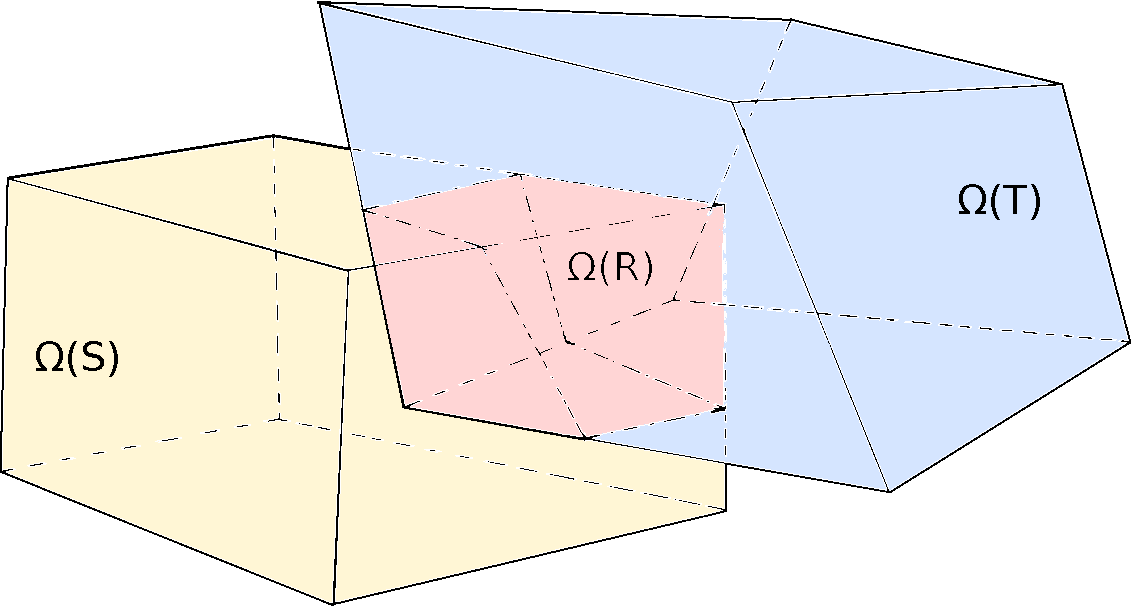
\includegraphics[width=4in]{overlapping_domain.pdf}
  \caption{Shared domain example. $\Omega(S)$ (yellow) is the source
    geometry, $\Omega(T)$ (blue) is the target geometry, and
    $\Omega(R)$ (red) is the shared domain.}
  \label{fig:shared_domain}
\end{figure}
The purpose of these mapping algorithms is to efficiently generate a
parallel topology map and the associated parallel communication plan
that can carry out the data transfer repeatedly with the minimum
required number of parallel messages and and data. A parallel topology
map is an operator, $M$, that defines the translation of a field,
$F(s): \mathbb{R}^D \rightarrow \mathbb{R}^N$, from a source spatial
and parallel domain, $\Omega_S$, to a field, $G(t): \mathbb{R}^D
\rightarrow \mathbb{R}^N$, in the target spatial and parallel domain
$\Omega_T$, such that $G(t)\leftarrow M(F(s))$ and $M: \mathbb{R}^N
\rightarrow \mathbb{R}^N, \forall r \in [\Omega_S \cap \Omega_T]$,
where $N$ is the dimensionality of the field and $D$ the
dimensionality of the spatial domain. It then follows that the
geometric rendezvous is defined as a geometric-based parallel
redistribution of the original source and target geometries defined
over the region $\Omega_R = \Omega_S \cap \Omega_T$.

These maps are generated by creating source/target pairs found by
searching the rendezvous decomposition. For each target object for
which data is desired, the rendezvous decomposition is searched with
that object to find the corresponding source object. In the case of
finite element interpolation, the target object would be a quadrature
point in the target finite element mesh and the source object would be
a source element in the source finite element mesh that contains the
target point. The map would then drive the field evaluation,
$G(t)\leftarrow M(F(s))$, for all source/target pairs. Embedded within
the map is a communication plan that describes the communication
sequence for transferring the data from the source geometry to the
target geometry. Once the field evaluations are complete, the
communication sequence moves that data from the source geometry
decomposition to the target geometry decomposition to complete the
data transfer and the application to the map operator.

\Subsection{Extension to General Geometries}
\label{subsec:general_geometry}

To handle software components that have a geometric entity-based
representation (e.g. a subchannel code discretized with a control
volume approach representing the geometry), the above algorithms have
been extended to operate on a general geometric description. The
mesh-based algorithm above is purely geometric, with each element in
the mesh treated as a separate geometric entity. If this is the case,
then other geometries such as annular rings, cubes, or any other
irregular shapes should apply to the algorithm. To extend the above
algorithm, we require a geometric entity to provide a small set of
information including point inclusion tests, the bounding box of the
entity, centroid, dimensionality. With this information, the RCB
partitioning can be generated and the geometry repartitioned to the
rendezvous decomposition. With the repartitioned geometry data we can
then perform a proximity search followed by the more expensive point
inclusion checks.

Given these new search structures, variations of the algorithms
presented in \cite{Plimpton_2004} can be extended beyond mesh-based
interpolation. DTK includes a geometric interpolation algorithm, very
similar to the original algorithm where data is applied to points in
the domain based on the field discretization in the geometry rather
than mesh elements. Geometry-to-geometry transfers are available when
the two physics components being coupled derive their geometric
description from the same source. This is useful in cases such as
transferring fuel temperatures from a geometric zone in one physics
application to the same geometric zone in another
application. Finally, for cases where volume-averaged quantities are
desired, typically an integral is evaluated over some volume of
space. To support these operations, DTK contains algorithms for
integrating mesh-based fields over the geometry that the mesh has
discretized.

%%---------------------------------------------------------------------------%%
\Section{DATA TRANSFER EXAMPLE USE CASES}
\label{sec:examples}

This section demonstrates important DTK use cases for CASL.  A goal of
the CASL program \cite{u.s._department_of_energy_casl_2011} is to
develop an advanced simulator capability for a pressurized light water
reactor core.  To achieve this, two large-scale parallel codes have
been coupled using DTK, a thermal hydraulics (TH) code
\cite{drekar_cfd} and a neutronics (NE) code \cite{denovo_2010}.  The
TH code performs a multiphysics conjugate heat transfer simulation
where energy conservation equation is solved in the fuel pins and
energy, momentum and mass conservation equations are solved in the
fluid surrounding the fuel pins.  The TH simulation uses fully coupled
fully implicit Newton-Krylov solvers with algebraic multigrid
preconditioning \cite{shadid_2006}.  In this coupling, DTK is
leveraged to transfer data in parallel between the codes and a simple
block Gauss-Siedel iteration loop is used to converge the global
coupled system.  Both codes have been demonstrated to run on
leadership class machines with greater than 100,000 cores.

The solution is spatially distributed across processes, requiring the
use of DTK to identify and execute an efficient communication plan
data transfer.  For NE to TH coupling, the NE code supplies source
terms used by the energy conservation equation in the fuel pins of the
TH code.  A point-to-point data transfer is required where where the
TH code requires source term values at the quadrature points for the
finite element integration.  For TH to NE coupling, the TH code
supplies average temperatures for a section of the fuel pin to the NE
code for the cross-section calculations.  An integral assembly
transfer is used to provide cell integrated contributions to the total
average temperature for the geometric entity (fuel pin section).
Sample 2D verification simulations from this work are provided in the
following section.

\Subsection{Data Transfer Verification}
\label{subsec:cht}

A simplified form of the full physics simulation was used to verify
parallel data transfer.  An analytic solution for the source term was
prescribed in the NE code and transferred to the TH code.  The
simulation was run on 10 cores with TH using 5 cores and NE using the
remaining 5 cores.  Figure \ref{fig:parallel_decomposition}
\begin{figure}[ht!]
  \centering
  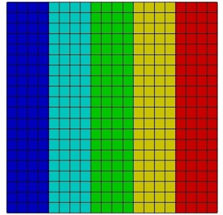
\includegraphics[width=2.0in]{neutronics_parallel_decomp.png}
  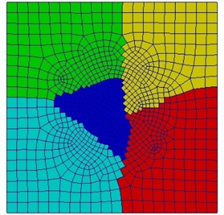
\includegraphics[width=2.0in]{cfd_parallel_decomp.png}
  \caption{Parallel decomposition.  The colors indicate ownership of
    the element by a core.  In this example, a 10 core job is run with
    the CFD and neutronics applications each owning 5 cores on
    separate processor spaces.}
  \label{fig:parallel_decomposition}
\end{figure}
 shows the parallel decomposition for each application code.  Note
 that NE uses a structured mesh while the TH uses an unstructured mesh
 as shown in Figure~\ref{fig:domain} on the left. Results showed that
 data was transferred correctly with machine precision accuracy using
 DTK.  A plot of the function verification function (source = $x*y$)
 is shown in Figure \ref{fig:domain} on the right.
\begin{figure}[ht!]
  \centering 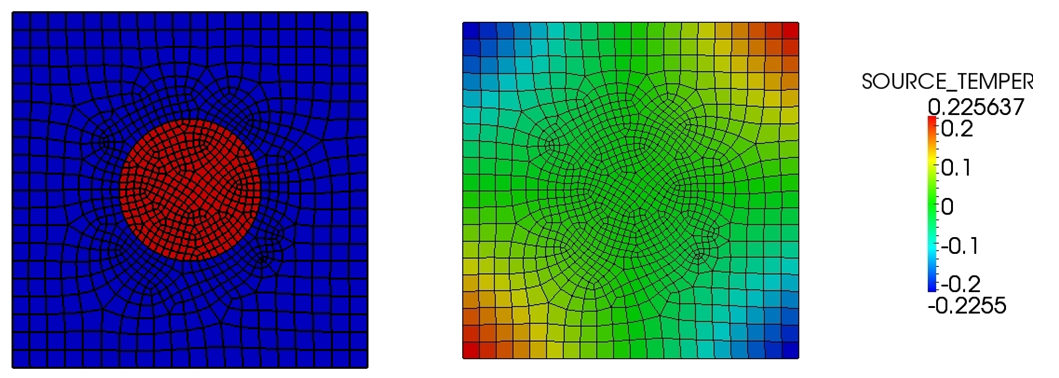
\includegraphics[width=6.0in]{cht_results.png}
  \caption{(Left) Verification simulation domain space consisting of a
    top-down view of a single fuel pin surrounded by a fluid
    region. The blue region represents the fluid area and the red
    region represents the solid fuel pin. (Right) Multiphysics domain
    space.}
  \label{fig:domain}
\end{figure}

%%---------------------------------------------------------------------------%%
\Section{PARALLEL SCALING STUDY}
\label{sec:scaling_study}

As indicated by the CASL use cases above, the current physics codes
leveraged scale to leadership class computing facilities. A typical
use case of DTK in these cases is searching a mesh with a set of
points and applying field data to those points through function
evaluations. For this use case, a scaling study of the mesh-based DTK
implementation of the rendezvous algorithm for data transfer was
performed utilizing the Jaguar Cray XK6 system at Oak Ridge National
Laboratory. For each study, a tri-linear hexahedron mesh was generated
and decomposed across the parallel domain. Each partition had one
element in the z direction while the x and y directions were varied to
produce the desired number of elements in the partition. All
partitions in each scaling study are square. This mesh is searched
with random points generated by sampling the x and y directions across
the global mesh domain.  By striding the random number seed used to
generate the point coordinates, each process will have a unique set of
random points it is searching for. For each scaling study, every
process generated the same number of random points as the number of
elements on that process, ensuring that a dense, all-to-all
communication operation will be required for mapping and data
transfer. Once the points are mapped to the mesh, the data transfer
routine applies the process rank in which they were found and
transfers it back to the original owning process for the point. In
this way, because of the simple partitioning used for the scaling
studies, the results of the data transfer to the random points can be
independently verified by checking the applied data against the
expected mesh process rank.

\Subsection{Weak Scaling}
\label{subsec:weak_scaling}
For the weak scaling study, the number of hexahedrons and random
points per partition were fixed to $1 \times 10^4$. The number of
cores used varied from 16 to 115,072. Figure~\ref{fig:weak_scaling}
gives the results of the weak scaling study. The largest case reported
here uses 115,072 cores and required 10.44 minutes for map generation
and 0.48 seconds for data transfer with a mesh size of $1.15 \times
10^9$ elements. It is clear from the weak scaling study that at high
numbers of processors communication latency begins to dominate for
this dense all-to-all problem as described above. However, it is worth
noting that once the mapping is complete, wall time for the actual
transfer of the data is several orders of magnitude less.

\begin{figure}[ht!]
  \centering 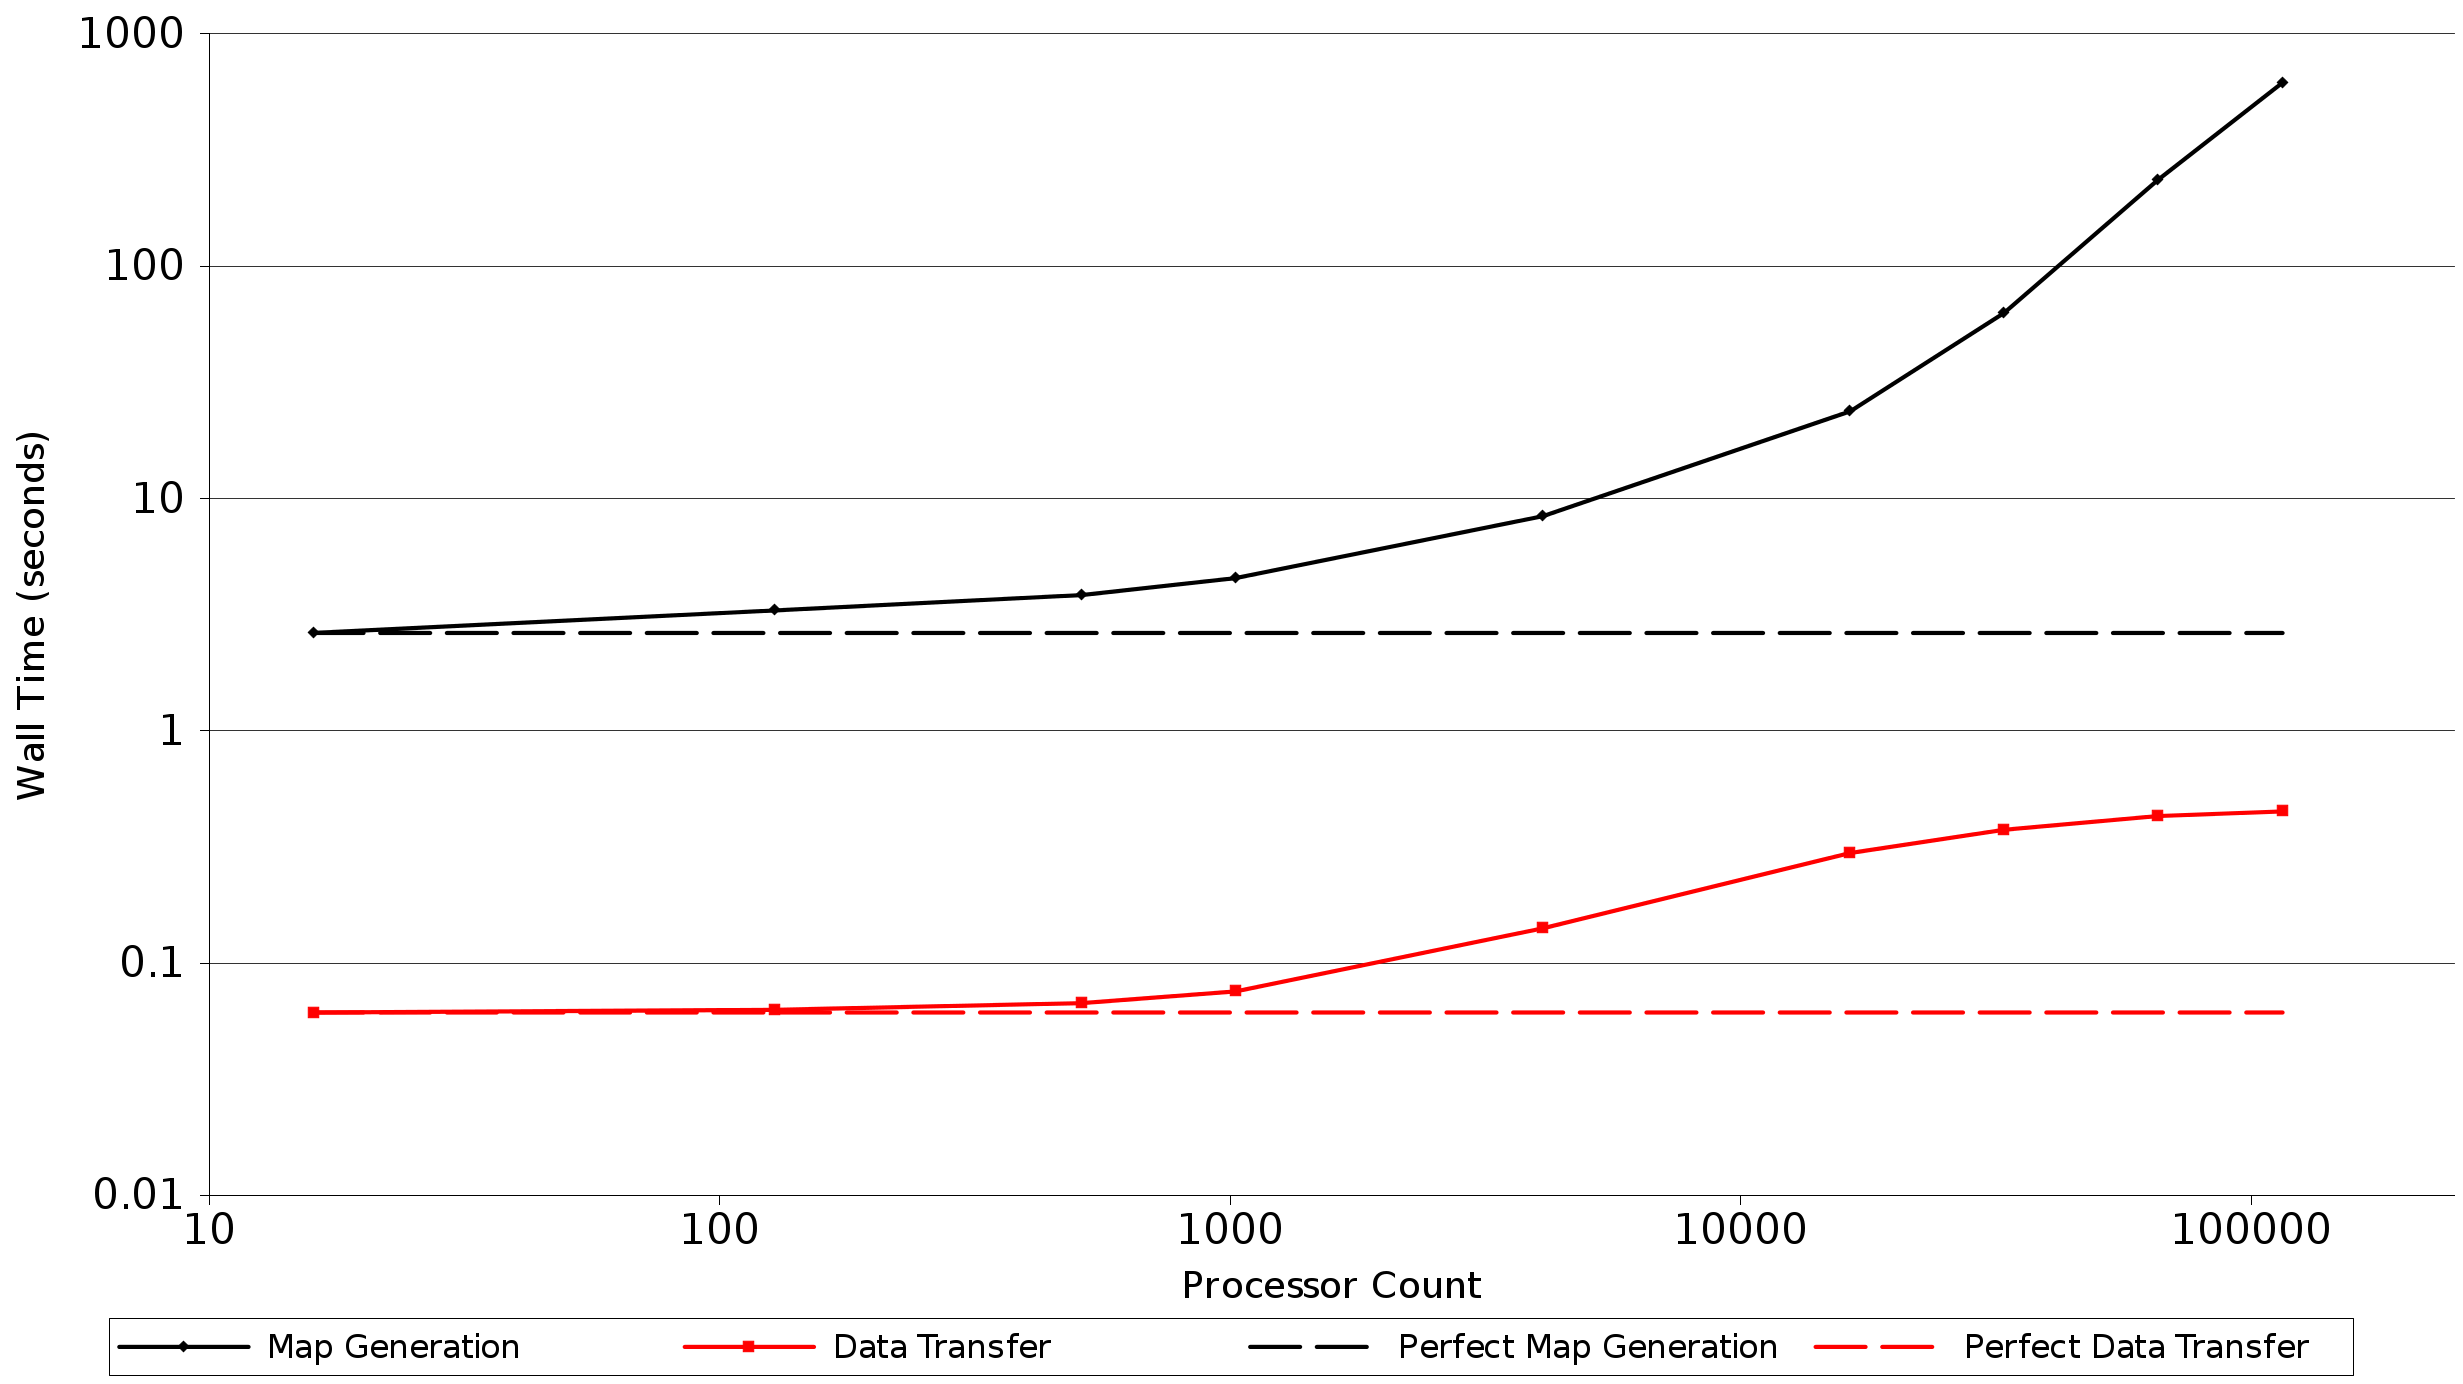
\includegraphics[width=5.5in]{WeakScaling.png}
  \caption{Weak scaling study results. The solid black curve reports
    the wall time to generate the mapping vs. number of processors
    while the solid red curve reports the wall time to transfer the
    data vs. number of processors. The dashed lines give perfect weak
    scaling the map generation (black) and the data transfer (red).}
  \label{fig:weak_scaling}
\end{figure}

Table~\ref{tab:weak_scaling} gives the raw data for the weak scaling
study. We note here that both the map generation time and the data
transfer time are relatively load balanced with average compute times
reported near the maximum compute time. In addition it should be noted
that for even the largest case at 115,072 cores the wall time is not
prohibitively large with the map generation routine requiring
approximately 10.44 minutes and the data transfer routine requiring
less than half a second.

The efficiency values for the map generation and data transfer
routines are also reported in Table~\ref{tab:weak_efficiency} with the
16 core case used as the reference computation. In correlation with
the data presented in Table~\ref{tab:weak_scaling}, the efficiencies
are observed to be low above 1,000 cores for this dense all-to-all
communication problem. For more physical coupling problems where the
communication is expected to be much sparser, this gives and idea of
just how sparse that communication must be for this algorithm to scale
well.

\begin{table}[htpb!]
  \begin{center}
    \begin{tabular}{llllllll}\hline\hline
      \multicolumn{1}{l}{} & \multicolumn{1}{l}{Global} &
      \multicolumn{1}{l}{Map} & \multicolumn{1}{l}{Map} &
      \multicolumn{1}{l}{Map} & \multicolumn{1}{l}{Transfer} &
      \multicolumn{1}{l}{Transfer} &
      \multicolumn{1}{l}{Transfer}\\ \multicolumn{1}{l}{Cores} &
      \multicolumn{1}{l}{Elements} & \multicolumn{1}{l}{Min (s)} &
      \multicolumn{1}{l}{Max (s)} & \multicolumn{1}{l}{Average (s)} &
      \multicolumn{1}{l}{Min (s)} & \multicolumn{1}{l}{Max (s)} &
      \multicolumn{1}{l}{Average (s)}\\ \hline\hline %% 16 & 1.600E+05
      & 2.63 & 2.65 & 2.635 & 0.06 & 0.07 & 0.062 \\ 128 & 1.280E+06 &
      3.25 & 3.31 & 3.30 & 0.06 & 0.07 & 0.063 \\ 512 & 5.120E+06 &
      3.58 & 3.86 & 3.84 & 0.06 & 0.08 & 0.067 \\ 1,024 & 1.024E+07 &
      3.98 & 4.53 & 4.48 & 0.06 & 0.09 & 0.076 \\ 4,096 & 4.096E+07 &
      6.54 & 8.51 & 8.39 & 0.13 & 0.15 & 0.141 \\ 16,384 & 1.638E+08 &
      15.98 & 27.0 & 23.73 & 0.28 & 0.32 & 0.296 \\ 32,768 & 3.277E+08
      & 40.03 & 68.18 & 62.88 & 0.36 & 0.39 & 0.375 \\ 65,536 &
      6.554E+08 & 214.69 & 239.21 & 234.76 & 0.41 & 0.45 & 0.429
      \\ 115,072 & 1.151E+09 & 570.12 & 626.51 & 616.675 & 0.42 & 0.48
      & 0.450 \\ \hline\hline
    \end{tabular}
  \end{center}
  \caption{\sl Weak scaling study data with the local problem size
    fixed to 1.0E4 elements/points. All times reported in
    seconds. Minimum, maximum, and average timing values are global
    and computed using the results from all processes.}
  \label{tab:weak_scaling}
\end{table}

\begin{table}[htpb!]
  \begin{center}
    \begin{tabular}{lll}\hline\hline
      \multicolumn{1}{c}{Cores}& \multicolumn{1}{c}{Map Efficiency} &
      \multicolumn{1}{c}{Transfer Efficiency}\\\hline\hline 16 & 1.000
      & 1.000 \\ 128 & 0.800 & 0.974 \\ 512 & 0.687 & 0.911 \\ 1,024 &
      0.581 & 0.812 \\ 4,096 & 0.314 & 0.434 \\ 16,384 & 0.111 & 0.206
      \\ 32,768 & 0.042 & 0.164 \\ 65,536 & 0.011 & 0.143 \\ 115,072 &
      0.004 & 0.136 \\ \hline\hline
    \end{tabular}
  \end{center}
  \caption{\sl Weak scaling efficiencies. The 16 process case was used
    as the reference case.}
  \label{tab:weak_efficiency}
\end{table}

Compared to the weak scaling results observed by Plimpton and
colleagues for a similar dense communication problem
\cite{Plimpton_2004}, these results show the same qualitative behavior
(see figure 7 in the reference). As the Jaguar system improves on all
aspects of machine performance over those used in the 2004 work, it is
expected that larger problems may be solved before the bandwidth
limiting behavior is observed.

\Subsection{Strong Scaling}
\label{subsec:strong_scaling}
For the strong scaling study, the global number of hexahedrons and
random points were fixed to $1 \times 10^8$ with the number of cores
varied from 256 to 65,536. Figure~\ref{fig:strong_scaling} gives the
results of the strong scaling study. Again, we note for the all-to-all
communication pattern required to map the random points that latency
again begins to dominate when a few thousand cores are used while the
data transfer scaling is excellent. The raw data for this study is
presented in Table~\ref{tab:strong_scaling}. We see again that the
algorithm is relatively load balanced with average compute times near
the maximum reported compute times for the map generation
operation. Table~\ref{tab:strong_efficiency} gives the efficiencies
computed for the strong scaling study with the 256 processor case used
as the reference.

\begin{figure}[htpb!]
  \centering 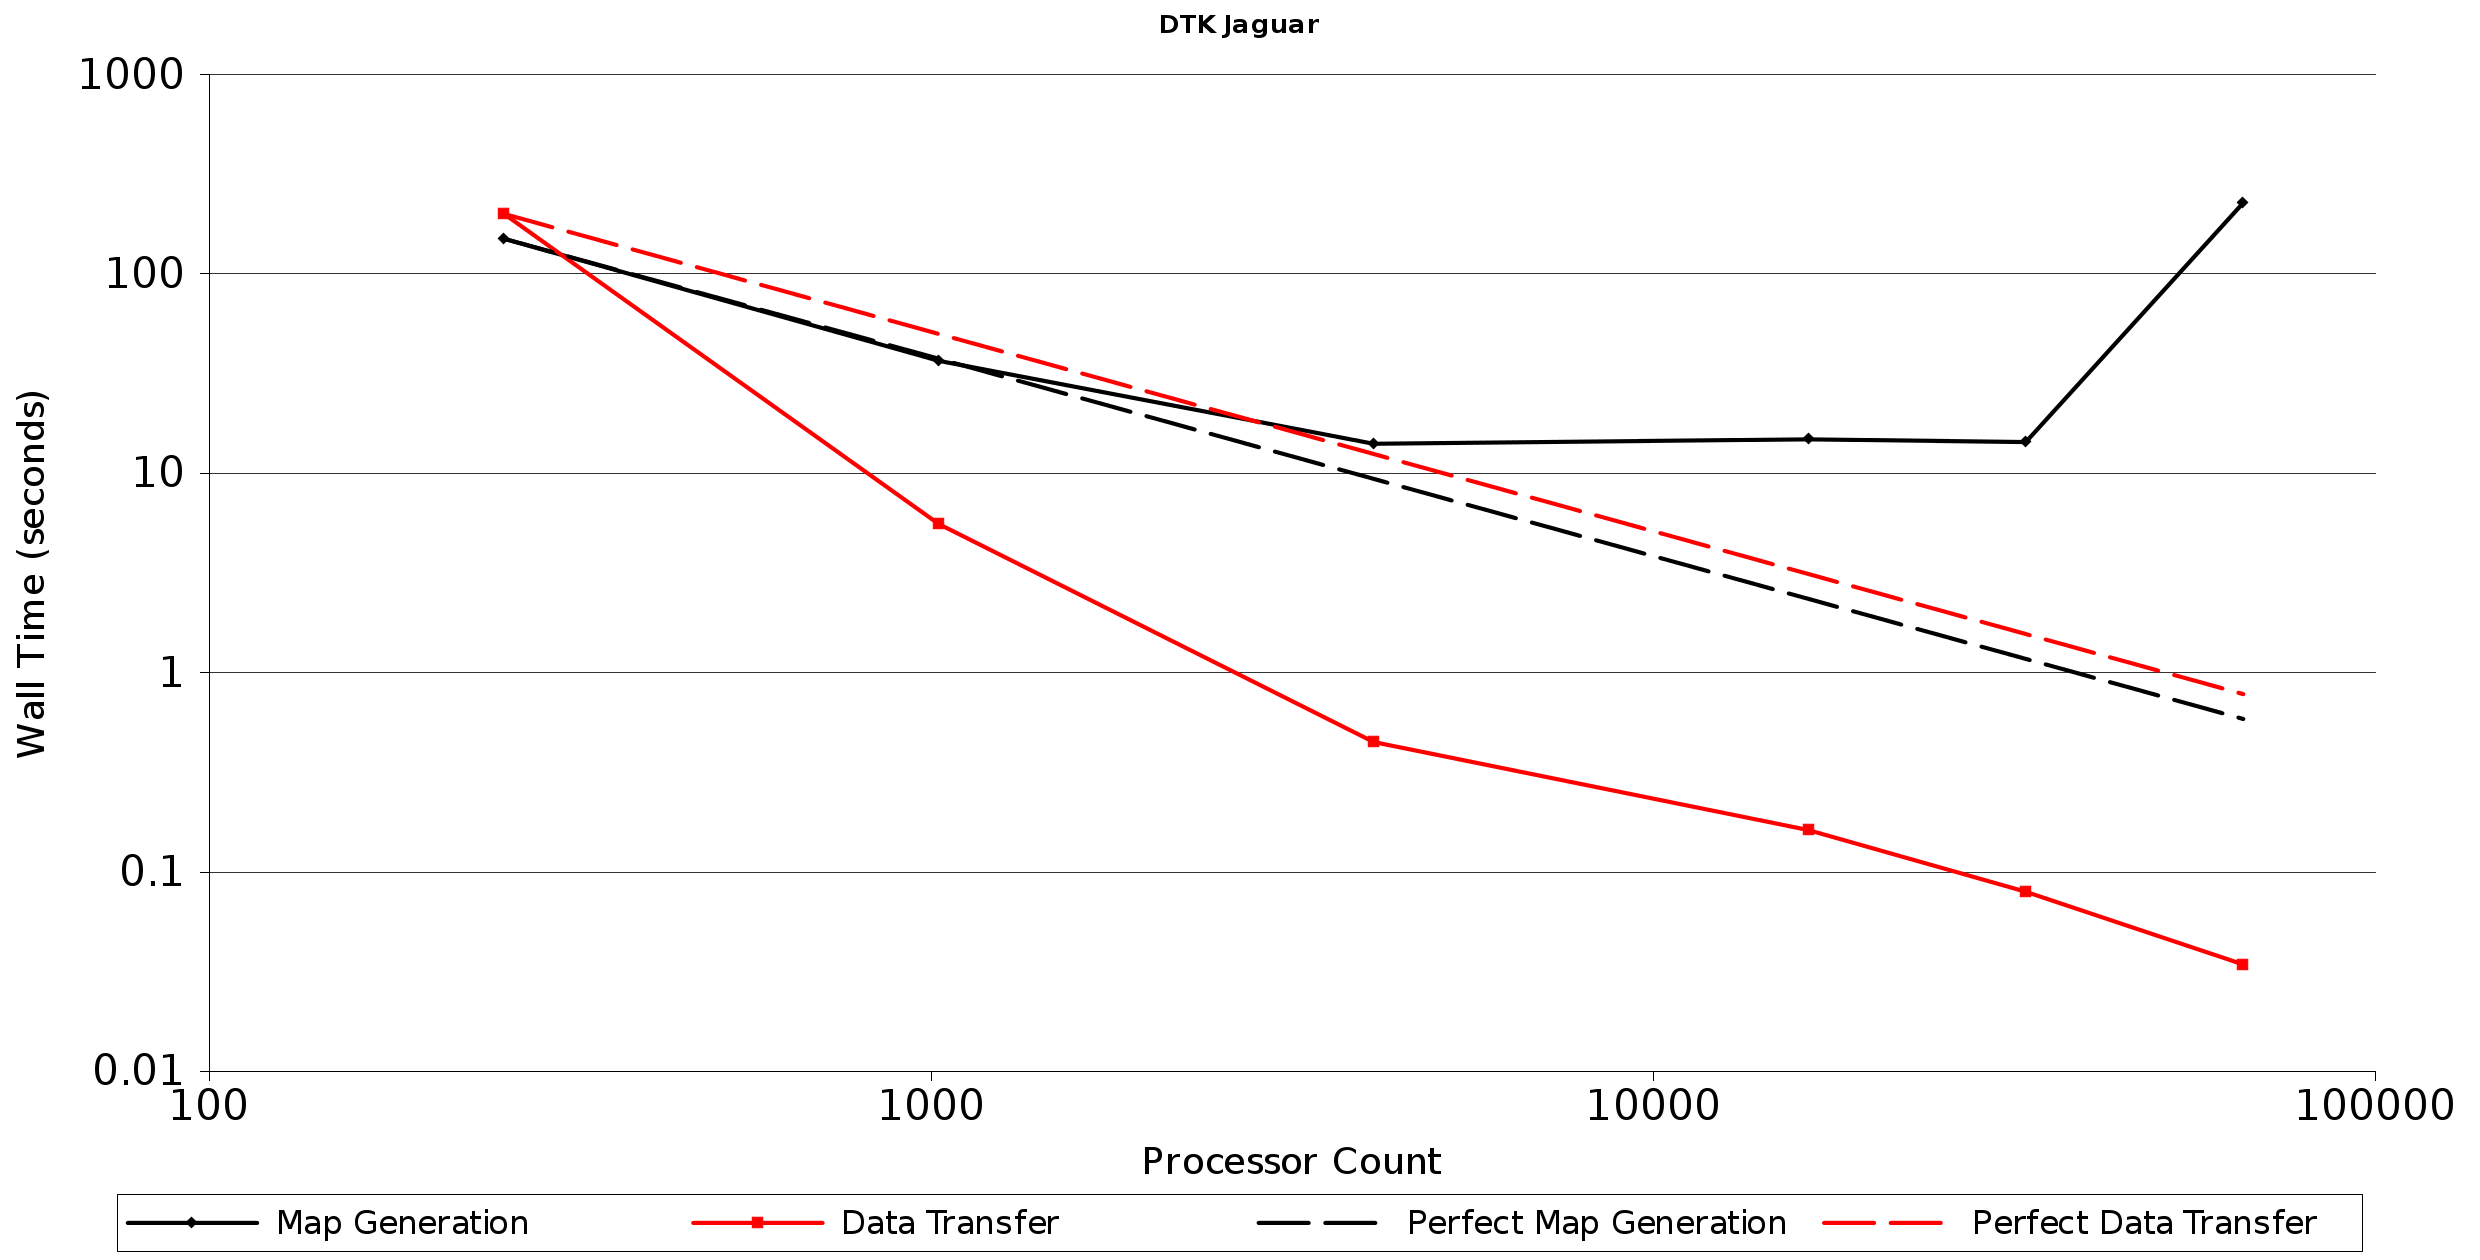
\includegraphics[width=5.5in]{StrongScaling.png}
  \caption{Strong scaling study results. The solid black curve reports
    the wall time to generate the mapping vs. number of processors
    while the solid red curve reports the wall time to transfer the
    data vs. number of processors. The dashed lines give perfect
    strong scaling the map generation (black) and the data transfer
    (red).}
  \label{fig:strong_scaling}
\end{figure}

\begin{table}[htpb!]
  \begin{center}
    \begin{tabular}{llllllll}\hline\hline
      \multicolumn{1}{l}{}& \multicolumn{1}{l}{Local} &
      \multicolumn{1}{l}{Map} & \multicolumn{1}{l}{Map} &
      \multicolumn{1}{l}{Map} & \multicolumn{1}{l}{Transfer} &
      \multicolumn{1}{l}{Transfer} &
      \multicolumn{1}{l}{Transfer}\\ \multicolumn{1}{l}{Cores} &
      \multicolumn{1}{l}{Elements} & \multicolumn{1}{l}{Min (s)} &
      \multicolumn{1}{l}{Max (s)} & \multicolumn{1}{l}{Average (s)} &
      \multicolumn{1}{l}{Min (s)} & \multicolumn{1}{l}{Max (s)} &
      \multicolumn{1}{l}{Average (s)}\\ \hline\hline %% 256 & 3.91E+05
      & 149.58& 150.04 & 149.883 & 198.99 & 199.81 & 199.72 \\ 1,024 &
      9.77E+04 & 36.08 & 36.68 & 36.60 & 5.52 & 5.59 & 5.55 \\ 4,096 &
      2.44E+04 & 12.12 & 14.18 & 14.0558 & 0.37 & 0.45 & 0.04
      \\ 16,384 & 6.10E+03 & 9.16 & 15.75 & 14.787 & 0.15 & 0.18 &
      0.162 \\ 32,768 & 3.05E+03 & 7.42 & 17.92 & 14.33 & 0.06 & 0.10
      & 0.080 \\ 65,536 & 1.53E+03 & 205.54 & 232.01 & 227.07 & 0.02 &
      0.05 & 0.034 \\ \hline\hline
    \end{tabular}
  \end{center}
  \caption{\sl Strong scaling study data. All times reported in
    seconds. Minimum, maximum, and average timing values are global
    and computed using the results from all processes.}
  \label{tab:strong_scaling}
\end{table}

\begin{table}[htpb!]
  \begin{center}
    \begin{tabular}{lll}\hline\hline
      \multicolumn{1}{c}{Cores}& \multicolumn{1}{c}{Map Efficiency} &
      \multicolumn{1}{c}{Transfer Efficiency}\\\hline\hline %% 256 &
      1.000 & 1.000 \\ 1,024 & 1.024 & 8.989 \\ 4,096 & 0.666 & 27.84
      \\ 16,384 & 0.158 & 19.24 \\ 32,768 & 0.082 & 19.62 \\ 65,536 &
      0.003 & 22.71 \\ \hline\hline
    \end{tabular}
  \end{center}
  \caption{\sl Strong scaling efficiencies. The 256 process case was
    used as the reference case.}
  \label{tab:strong_efficiency}
\end{table}

%%---------------------------------------------------------------------------%%
\Section{CONCLUSIONS}

We have presented the Data Transfer Kit, a new tool for parallel data
transfer for multiphysics applications. The concept of geometric
rendezvous is used to provide a collection of mesh and geometry-based
mappings for data transfer in shared domain problems. Initial scaling
studies have been completed for the Data Transfer Kit on the Jaguar
Cray XK6 system. Their results show comparable qualitative behavior to
the literature results with improved performance due to the more
advanced computational resources available with good scaling for the
data transfer operation at $O(1 \times 10^5)$ cores. However, for the
dense communication patterns required to complete the scaling study
problem, poor weak scaling results are still observed above $O(1
\times 10^4)$ cores for the mapping operation. For data transfer
problems where the underlying mesh or geometry does not change, the
wall times observed for the mapping algorithm to be performed may not
be prohibitive as that operation will only be performed once during a
setup phase for the problem. Once the map is generated, it and the
resulting parallel communication plan can be used repeatedly in the
data transfer operation with excellent scaling and minimal wall time
observed for meshes of $O(1 \times 10^9)$ elements.

It is expected for more physical data transfer problems that the
overall communication pattern will be significantly sparser than the
problem presented here. Because of this, scaling for the mapping
algorithm is expected to improve for more physical problems. Further
scaling studies will be required to test this hypothesis. In addition,
Data Transfer Kit has the potential to be extended to provide
surface-to-surface mappings for interface data transfers.


%%---------------------------------------------------------------------------%%
\section*{ACKNOWLEDGEMENTS}

This work was performed under funding provided by the Consortium for
Advanced Simulation of Light Water Reactors (CASL). The authors would
like to thank the CASL Virtual Reactor Integration (VRI) development
team for their assistance over the course of development of DTK and
the Oak Ridge Leadership Computing Facility (OLCF) for providing
computational resources and support.

%%---------------------------------------------------------------------------%%
%\Section*{REFERENCES}
\setlength{\baselineskip}{12pt}
\bibliographystyle{ieeetr}
\bibliography{references}

\end{document}


